\chapter{Theory and motivations}
\label{CHAPTER:TheoryAndMotivations}

\glsresetall % Resetting all acronyms

%%%%%%%%%%%%%%%%%%%%%%%%%%%%%%%%%%%%%%%%%%%%%%%%%%%%%%%%%%%%%%%%%%%%%%%%%%%%%%%%%%%%%%%
%%% SECTION
%%%%%%%%%%%%%%%%%%%%%%%%%%%%%%%%%%%%%%%%%%%%%%%%%%%%%%%%%%%%%%%%%%%%%%%%%%%%%%%%%%%%%%%
\section{Standard Model of Particle Physics}

% Status: DONE

The \gls{SM} of particle physics is a quantum field theory that describes the electromagnetic, weak nuclear and strong forces and their interaction with matter. This theory is one of the most successful theories ever made and was able to describe data from a wide range of experimental measurements. Before its discovery in 2012 \cite{ARTICLE:ATLAS_HiggsDiscovery,ARTICLE:CMS_HiggsDiscovery} the Higgs boson was the only missing particle that was predicted by this theory and not yet found. 

Although its success, the \gls{SM} does not explain some phenomena observed in nature, like the presence of large quantity of \textit{dark matter} in the universe, or the even more mysterious \textit{dark energy}. The discovery of the Higgs boson could allow to probe the production of dark matter directly, through its decay into these elusive particles. This chapter briefly describes the theory behind the \gls{SM}, the Higgs mechanism, how to search for Higgs invisible decays.

%%%%%%%%%%%%%%%%%%%%%%%%%%%%%%%%%%%%%%%%%%%%%%%%%%%%%%%%%%%%%%%%%%%%%%%%%%%%%%%%%%%%%%%
%%% SUBSECTION
%%%%%%%%%%%%%%%%%%%%%%%%%%%%%%%%%%%%%%%%%%%%%%%%%%%%%%%%%%%%%%%%%%%%%%%%%%%%%%%%%%%%%%%
\subsection{Particles and forces}
\label{SUBSECTION:Theory_SM_ParticlesAndForces}



\begin{table}[!htb]
  \centering
  \begin{tabular}{|c|c|c|c|c|}
  \hline
  \multicolumn{5}{|c|}{Leptons (J=1/2)} \\
  \hline
  Generation & Particle Name & Symbol & Mass ($GeV/c^2$) & Q/e \\
  \hline
  \hline
  \multirow{2}{*}{$1^{st}$} & Electron          & e          &           0.000511    & 1 \\
                            & Electron Neutrino & $\nu_e$    & $< 3 \times 10^-9$    & 0 \\
  \hline
  \hline
  \multirow{2}{*}{$2^{nd}$} & Muon              & $\mu$      &              0.106    & 1 \\
                            & Muon Neutrino     & $\nu_\mu$  & $< 1.9 \times 10^-4$  & 0 \\
  \hline
  \hline
  \multirow{2}{*}{$3^{rd}$} & Tau               & $\tau$     & 1.777                 & 1 \\
                            & Tau Neutrino      & $\nu_\tau$ & $< 1.82 \times 10^-2$ & 0 \\
  \hline
  \end{tabular}
  \caption[List of leptons and their fundamental properties]{List of leptons and their fundamental properties}
  \label{TheoreticalIntroduction_LeptonProperties}
\end{table}

\begin{table}[!htb]
  \centering
  \begin{tabular}{|c|c|c|c|c|}
  \hline
  \multicolumn{5}{|c|}{Quarks (J=1/2)} \\
  \hline
  Generation & Particle Name & Symbol & Mass ($GeV/c^2$) & Q/e \\
  \hline
  \hline
  \multirow{2}{*}{$1^{st}$} & Up      & u & $1.5-3.3 \times 10^{-3}$ & -2/3 \\
                            & Down    & d &   $3.5-6 \times 10^{-3}$ &  1/3 \\
  \hline
  \hline
  \multirow{2}{*}{$2^{nd}$} & Charm   & c &                1.16-1.34 & -2/3 \\
                            & Strange & s &  $70-130 \times 10^{-3}$ &  1/3 \\
  \hline
  \hline
  \multirow{2}{*}{$3^{rd}$} & Top     & t &                  169-173 & -2/3 \\
                            & Bottom  & b &              $4.13-4.37$ &  1/3 \\
  \hline
  \end{tabular}
  \caption[List of quarks and their fundamental properties]{List of quarks and their fundamental properties}
  \label{TheoreticalIntroduction_QuarkProperties}
\end{table}

\begin{table}[!htb]
  \centering
  \begin{tabular}{|c|c|c|c|c|}
  \hline
  \multicolumn{4}{|c|}{Bosons} \\
  \hline
   Particle Name & Mass ($GeV$) &     Q/e & Spin \\
  \hline
  \hline
  Photon ($\gamma$) &                  0 &       0 &    1 \\
  \hline
  $W^\pm$           & $80.385 \pm 0.015$ & $\mp 1$ &    1 \\
  $Z^0$             & $91.1876\pm0.0021$ &       0 &    1 \\
  \hline
  Gloun (g)         &                  0 &       0 &    1 \\
  \hline
  \end{tabular}
  \caption[List of bosons and their fundamental properties]{List of force carrying bosons and their fundamental properties \cite{ARTICLE:PDG2014}.}
  \label{TABLE:Theory_SM_ParticlesAndForces_BosonProperties}
\end{table}


%%%%%%%%%%%%%%%%%%%%%%%%%%%%%%%%%%%%%%%%%%%%%%%%%%%%%%%%%%%%%%%%%%%%%%%%%%%%%%%%%%%%%%%
%%% SUBSECTION
%%%%%%%%%%%%%%%%%%%%%%%%%%%%%%%%%%%%%%%%%%%%%%%%%%%%%%%%%%%%%%%%%%%%%%%%%%%%%%%%%%%%%%%
\subsection{The Higgs mechanism}

Summary of the Higgs Mechanism. Should include
\begin{itemize}
 \item Motivations 
 \item Explanation of the mechanism itself
 \item Consequences 
 \item Possible decays
\end{itemize}

%%%%%%%%%%%%%%%%%%%%%%%%%%%%%%%%%%%%%%%%%%%%%%%%%%%%%%%%%%%%%%%%%%%%%%%%%%%%%%%%%%%%%%%
%%% SUBSECTION
%%%%%%%%%%%%%%%%%%%%%%%%%%%%%%%%%%%%%%%%%%%%%%%%%%%%%%%%%%%%%%%%%%%%%%%%%%%%%%%%%%%%%%%
\subsection{Searching for the SM Higgs boson}


\begin{figure}[htbp]
\subfloat[]{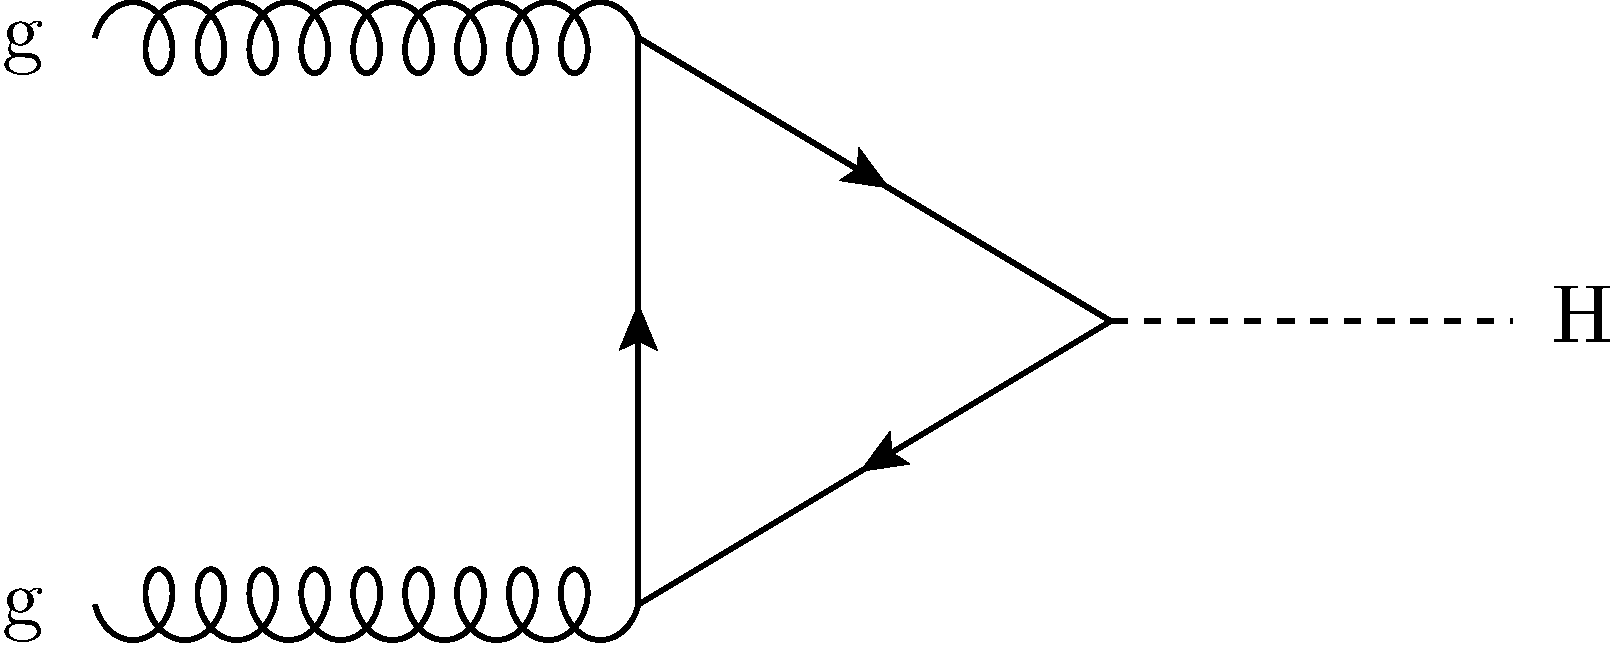
\includegraphics[width=0.45\textwidth]{Chapter01/Images/feynman_ggH.pdf}} \qquad
\subfloat[]{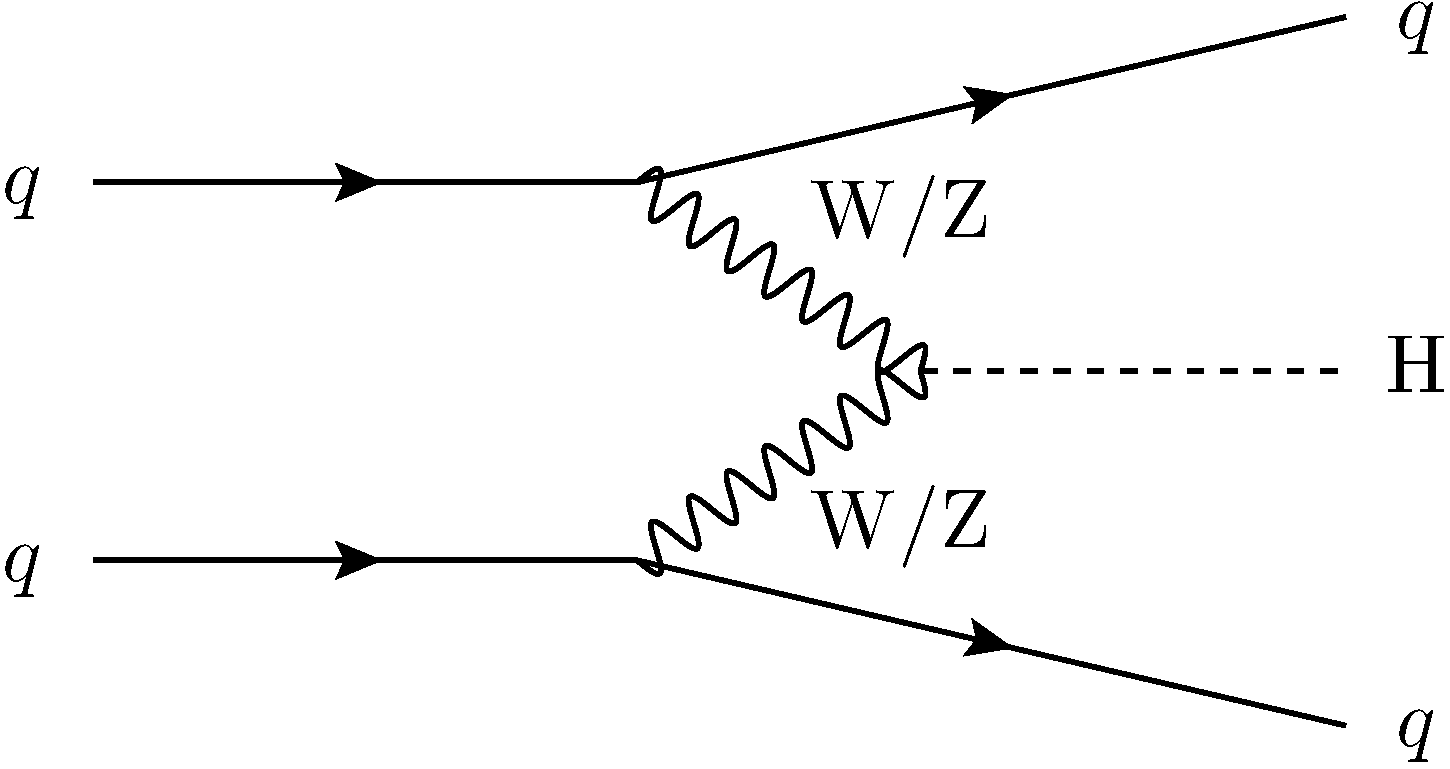
\includegraphics[width=0.45\textwidth]{Chapter01/Images/feynman_qqH.pdf}} \\
\subfloat[]{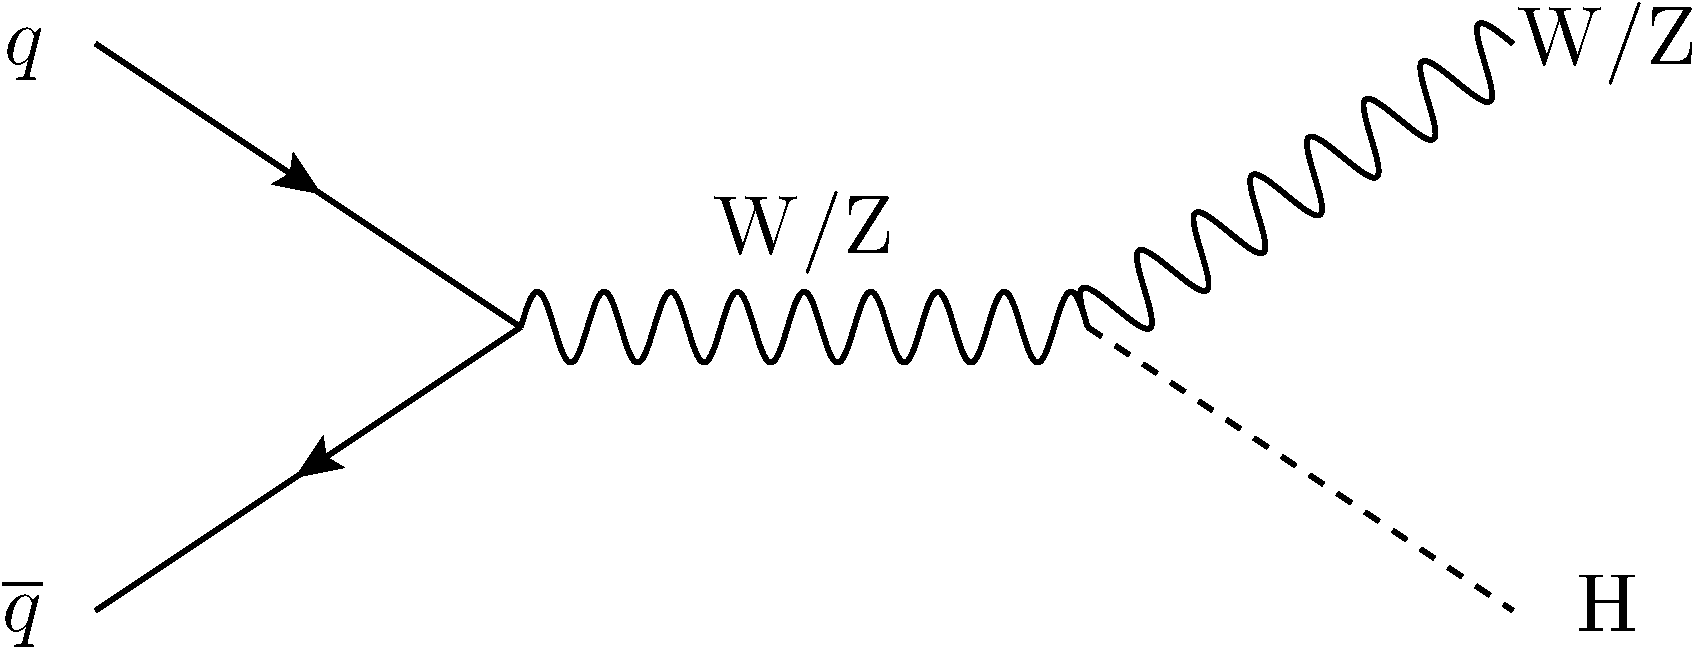
\includegraphics[width=0.45\textwidth]{Chapter01/Images/feynman_VH.pdf}}  \qquad
\subfloat[]{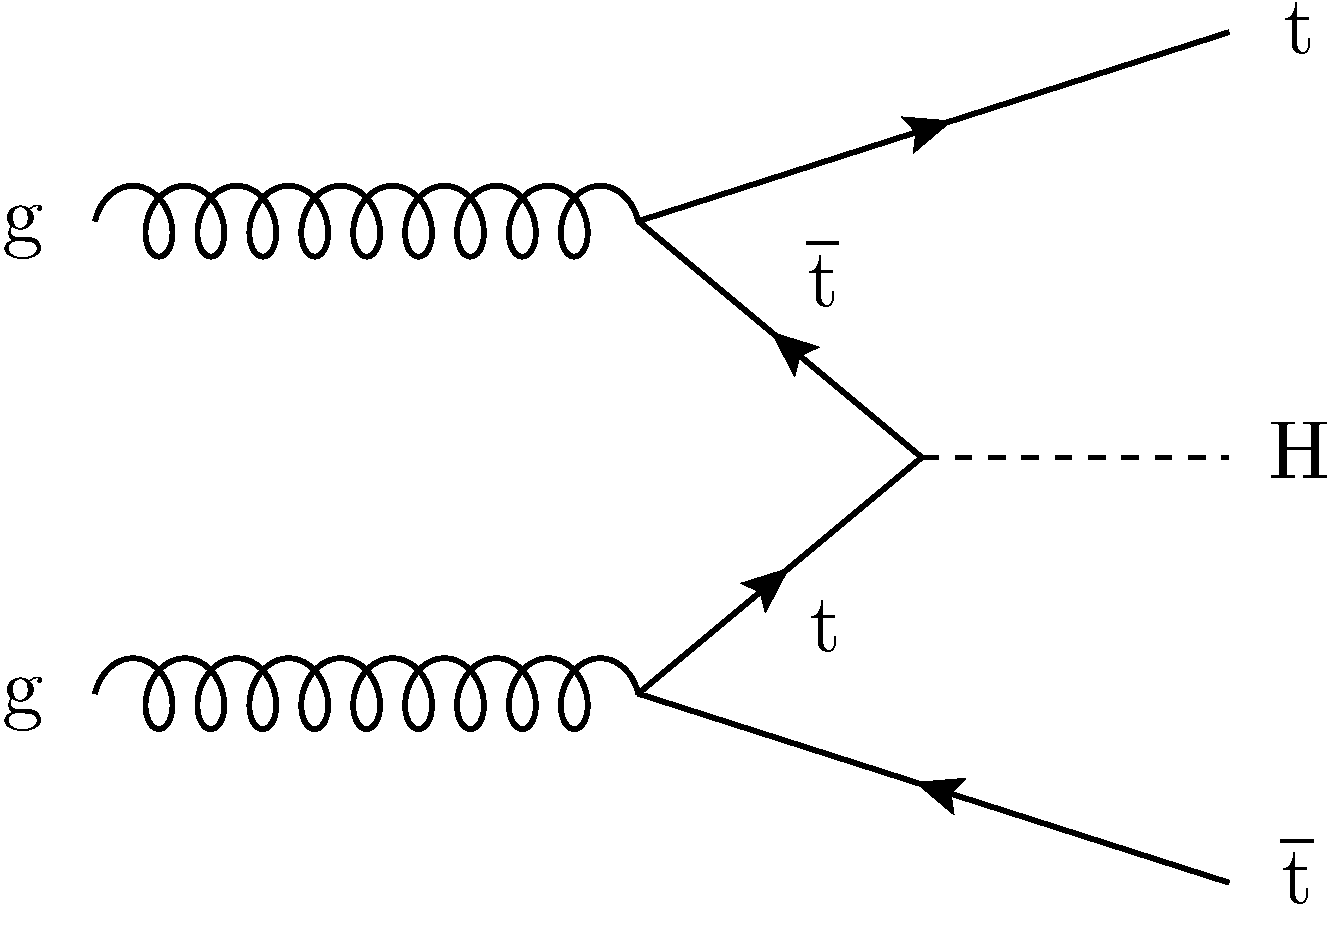
\includegraphics[width=0.45\textwidth]{Chapter01/Images/feynman_ttH.pdf}} \\
\caption[Feynman diagrams for the dominant production processes of the SM Higgs
boson.]{Feynman diagrams for the dominant production processes of the SM Higgs
boson. Shown is a) gluon fusion, b) vector boson fusion and
associated production with c) vector bosons and d) top quarks.}
\label{fig:SMFeynmanDiagrams}
\end{figure}

\begin{figure}[htbp]
 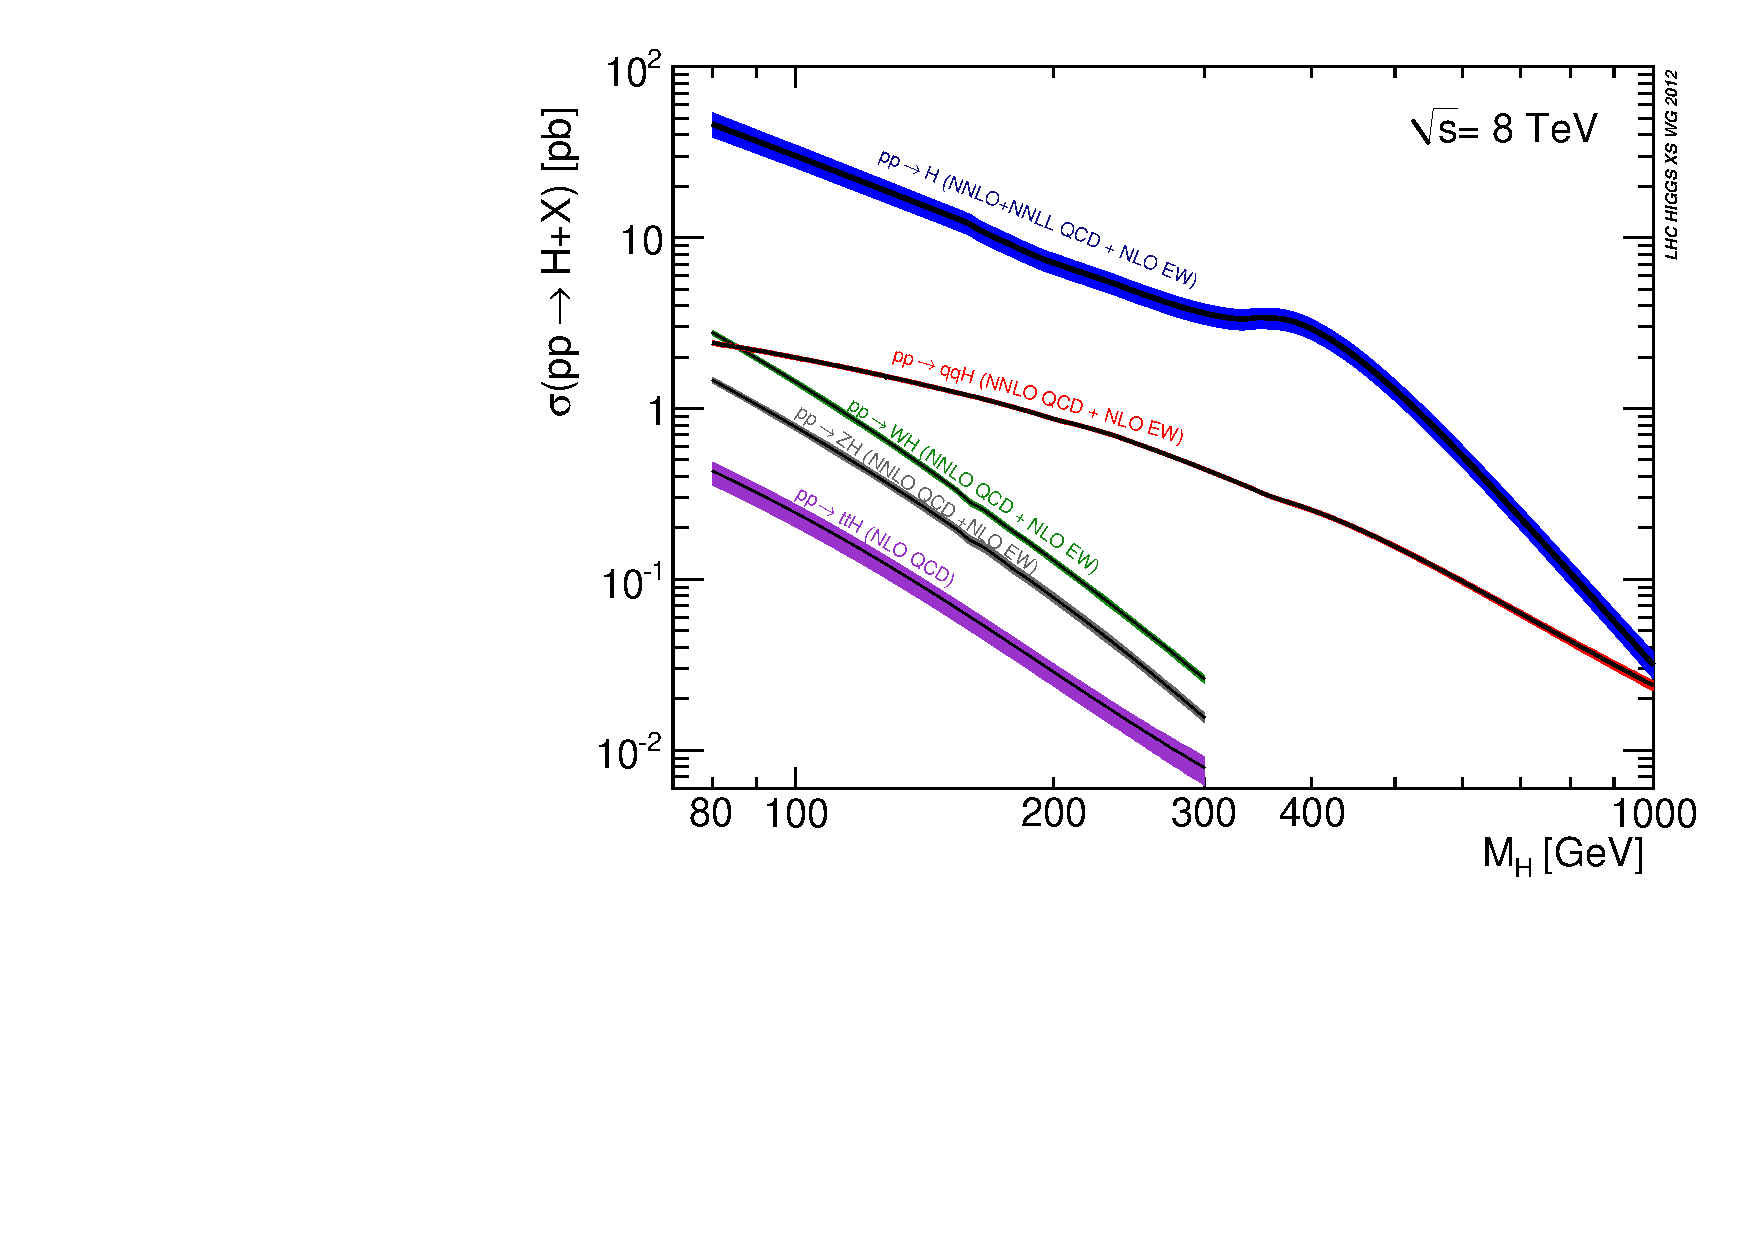
\includegraphics[width=0.7\textwidth]{Chapter01/Images/Higgs_XS_8TeV_lx.pdf}
\caption[Cross sections for Higgs production processes at $\sqrt{s}=8\,\TeV$ for
a range of Higgs boson masses.]{Cross sections for Higgs production processes at
$\sqrt{s}=8\,\TeV$ for a range of Higgs boson masses $m_{\PH}$~\cite{Heinemeyer:2013tqa}. Across the
mass range the gluon-fusion mode dominates, followed by the vector boson fusion
and associated production modes. The widths of the lines represent the
theoretical uncertainties on the cross section calculation.}
\label{fig:SMHiggsXS}
\end{figure}

\begin{figure}[htbp]
 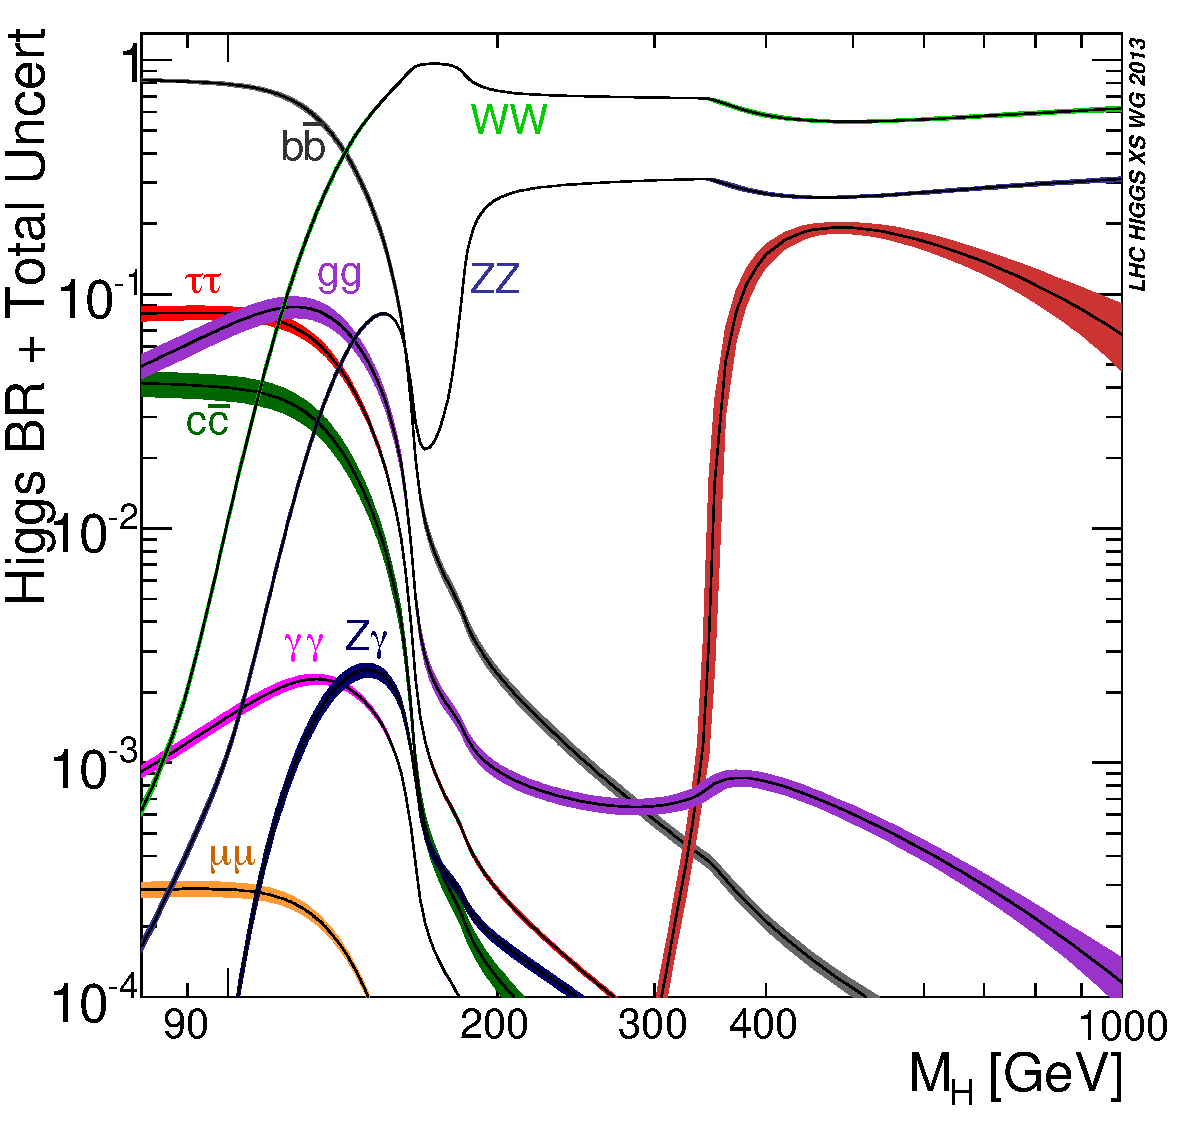
\includegraphics[width=0.6\textwidth]{Chapter01/Images/Higgs_BR.pdf}
\caption[Higgs boson branching ratios in the SM for a range of Higgs boson
masses.]{Higgs boson branching ratios in the SM for a range of Higgs boson
masses $m_{\PH}$ \cite{Heinemeyer:2013tqa}. At high masses, above their
kinematic thresholds, the $\PW\PW$,
$\PZ\PZ$ and $\ttbar$ (shown in red) decay modes dominate. 
At lower masses a wide range of different final states is possible. 
The widths of the lines represent the
theoretical uncertainties on the branching ratio calculation.}
\label{fig:SMHiggsBRs}
\end{figure}

\subsection{Higgs Invisible decays}

\colorbox{red}{
\begin{minipage}{0.95\linewidth}
TODO: 
\begin{itemize}
  \item Explain what are SM Higgs invisible decays.
  \item Go over the possibility of BSM invisible decays.
\end{itemize}

\end{minipage}
}

% Adding a bunch of references
\cite{ARTICLE:Higgs_SpontaneousSymmetryBreakdown}
\cite{BOOK:Griffiths}

